\documentclass{standalone}
\usepackage{mathrsfs}
\usepackage[x11names]{xcolor}
\usepackage{tikz, tkz-euclide}
\usepackage[american]{circuitikz}
\usepackage{siunitx}
\usepackage{textcomp}
\usetikzlibrary{arrows}
\begin{document}

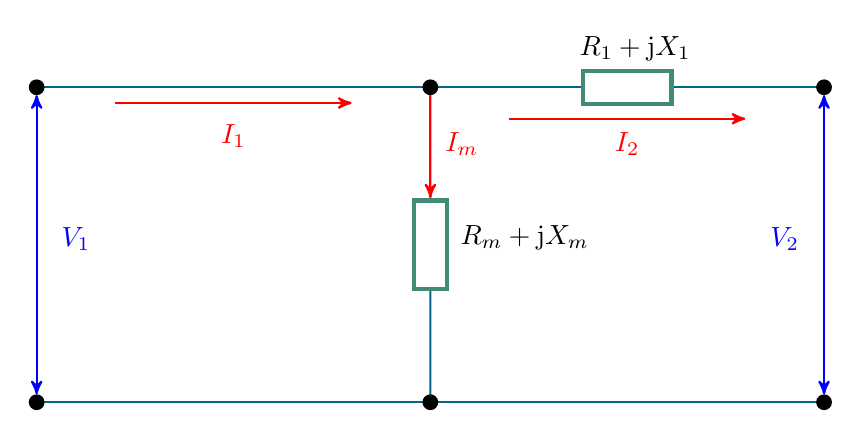
\begin{tikzpicture}[draw=DeepSkyBlue4,thick]
\draw (0,0) to (5,0);
\draw (5,0) to (10,0);
\draw (0,4) to (5,4);
\draw (5,0) to[european resistor, color=Aquamarine4] (5,4);
\draw (5,4) to[european resistor, color=Aquamarine4] (10,4);
\draw[draw opacity=0, fill=black] (0,0) circle (0.1);
\draw[draw opacity=0, fill=black] (0,4) circle (0.1);
\draw[draw opacity=0, fill=black] (5,0) circle (0.1);
\draw[draw opacity=0, fill=black] (5,4) circle (0.1);
\draw[draw opacity=0, fill=black] (10,0) circle (0.1);
\draw[draw opacity=0, fill=black] (10,4) circle (0.1);

\draw [<->,>=stealth',thick,blue] (0,0.1) -- (0,3.9);
\draw [<->,>=stealth',thick,blue] (10,0.1) -- (10,3.9);

\draw [->,>=stealth',thick,red] (1,3.8) -- (4,3.8);
\draw [->,>=stealth',thick,red] (6,3.6) -- (9,3.6);
\draw [->,>=stealth',thick,red] (5,3.9) -- (5,2.6);

\tkzLabelPoint[above,red](5.4,3){{\(I_{m}\)}}
\tkzLabelPoint[above,red](2.5,3.1){{\(I_{1}\)}}
\tkzLabelPoint[above,red](7.5,3){{\(I_{2}\)}}

\tkzLabelPoint[above,blue](0.5,1.8){{\(V_{1}\)}}
\tkzLabelPoint[above,blue](9.5,1.8){{\(V_{2}\)}}

\tkzLabelPoint[above](6.2,1.8){{\(R_{m}+\mathrm{j}X_{m}\)}}
\tkzLabelPoint[above](7.6,4.2){{\(R_{1}+\mathrm{j}X_{1}\)}}
\end{tikzpicture}
\end{document}
